



\chapter{Instalační manuál}
\label{append:instalace}

\section{Lokální vývojové prostředí}
Stručný návod jak spustit lokální vývojové prostředí. (psáno na OS Windows)\\
Další informace je případně možno nalézt také v Cookiecutter-django dokumentaci\footnote{Cookiecutter-django dokumentace \url{https://cookiecutter-django.readthedocs.io/en/latest/developing-locally.html}}

\label{append:instalace-local}
\begin{enumerate}
    \item Nainstalujte prerekvizity\\
    Je třeba si nainstalovat všechny potřebné aplikace - python3, git, postgreSQL databázi a Mailhog\footnote{Mailhog: \url{https://github.com/mailhog/MailHog}}. 
    
    \item Vytvořte virtuální prostředí\\
    Je dobrým zvykem umisťovat python projekty zvlášť, každý do vlastního virtuálního prostředí, aby se vzájemně nemohly ovlivňovat. Přejděte do složky kde budete chtít mít projekt umístěn a otevřete powershell. Nyní proveďte příkaz
    
    \texttt{\$ python3 -m venv virtualenv}
    
    kterým je vytvořeno virtuální prostředí ve složce \texttt{/virtualenv}. 
    
    \item Aktivujte virtuální prostředí\\
    Nyní je třeba toto prostředí v konzoli aktivovat pomocí příkazu
    
    \texttt{\$ ./virtualenv/Scripts/activate}
    
    V tuto chvíli by měl být vidět název Vašeho virtuálního prostředí v konzoli. Odteď jsou implicitně všechny příkazy vykonávány uvnitř tohoto prostředí.
    
    \item Naklonujte Github\footnote{Github: \url{https://github.com/}} repozitář\\
    Jelikož tato práce bude trvale umístěna na mém veřejném Github repozitáři, lze ho použít k naklonování souborů projektu. Spuštěním příkazu 
    
    \texttt{\$ git clone https://github.com/tmajerech/volebni\_kalkulacka.git}
    
    se v aktuálním adresáři vytvoří podadresář \texttt{volebni\_kalkulacka}, sloužící jako kořenový adresář aplikace a obsahující všechny potřebné soubory.
    

    \item Nainstalujte potřebné python moduly\\
    Následující příkazy změní složku do kořenového adresáře aplikace a spustí instalaci python balíčků z instalačního seznamu. Díky tomu je není třeba instalovat po jednom ručně. Příkazem \texttt{upgrade pip} je také nejprve nainstalována poslední verze python instalátoru balíčků.

    \texttt{\$ python3 -m pip install –upgrade pip}\\
    \texttt{\$ cd volebni\_kalkulacka}\\
    \texttt{\$ pip install -r requirements/local.txt}

    Pokud aplikaci instalujete na operačním systému Linux, můžete v této fázi narazit na problémy s některými MYSQL balíčky. Následující kroky by mohly pomoct:
    \begin{itemize}
        \item \texttt{sudo apt-get install libmysqlclient-dev}
        \item Pokud po instalaci předchozí závislosti přetrvávají chybové hlášky jako například \\
        \texttt{No such file or directory \#include "mysql/udf\_registration\_types.h"},\\
        je možnost vyzkoušet smazání "\texttt{mysql/}"\ z hlavičkového souboru který tuto chybu způsobuje - cesta k němu by měla být viditelná v samotném chybovém hlášení. Tímto způsobem je možno odstranit i některé další chyby, ale toto řešení doporučuji zvážit pouze jako úplně poslední a dočasné.
    \end{itemize}
    
    \item Nastavte připojení k databázi\\
    V kořenovém adresáři aplikace (volebni\_kalkulacka) vytvořte soubor \texttt{.env} do kterého vložíte následující nastavení. Hodnoty upravte podle vlastních. Konstantu \texttt{USE\_DOCKER} ponechte beze změny.
    \begin{verbatim}
    POSTGRES_HOST=localhost
    POSTGRES_PORT=5432
    POSTGRES_DB=volebnikalkulacka
    POSTGRES_USER=postgres
    POSTGRES_PASSWORD=root
    USE_DOCKER=NO
    \end{verbatim}
    
    \item Vytvořte databázové tabulky\\
    Následující příkaz v kořenovém adresáři spustí tzv. \texttt{databázové migrace}, které vytvoří všechny potřebné tabulky podle vytvořených modelů. 

    \texttt{\$ python3 manage.py migrate}

    \item Spusťte lokální server\\
    Příkazem
    
    \texttt{\$ npm run dev}
    
    je spuštěn lokální vývojový server spolu s automatickým obnovením stránky při úpravě v HTML šablonách a také automatickou kompilací a doplněním CSS po uložení změn v SASS souboru - v tomto případě bez nutnosti obnovení stránky. Po startu serveru by se mělo automaticky otevřít okno s aplikací. V případě neotevření automaticky by se měla aplikace nacházet na url \url{http://127.0.0.1:8000/}.
    
    \item Spusťte Mailhog lokální emailový server\\
    Je třeba spustit stažený mailhog \texttt{.exe} soubor, který v příkazové řádce spustí lokální emailový server. Příkazový řádek je třeba nechat otevřený po dobu využívání emailů, jelikož nemá žádnou paměť a po vypnutí ztratí všechny zachycené emaily. Po zapnutí naleznete rozhraní emailového klienta na adrese \texttt{http://localhost:8025/}
    
    \item Vytvořte administračního uživatele.\\
    Například pro možnost mazat závadné komentáře je třeba vytvořit tzv. \texttt{super uživatele}. K tomu slouží příkaz

    \texttt{\$ python3 manage.py createsuperuser}

    který už poté uživatele provede sám vytvářením.
    
    
\end{enumerate}




\section{Produkční prostředí}
\label{append:instalace-production}
Další informace je možné opět nalézt v dokumentaci pro Cookiecutter-django\footnote{Cookiecutter-django produkční nastavení: \url{https://cookiecutter-django.readthedocs.io/en/latest/deployment-with-docker.html}}

\begin{enumerate}
    \item Instalace prerekvizit\\
    Je třeba nainstalovat Python3, Git, Docker\footnote{Docker instalace: \url{https://docs.docker.com/get-docker/}}, Docker-compose\footnote{Docker-compose instalace: \url{https://docs.docker.com/compose/install/}}
    
    \item 
\end{enumerate}







\chapter{Databázový diagram}

\begin{sidewaysfigure}
    \centering
    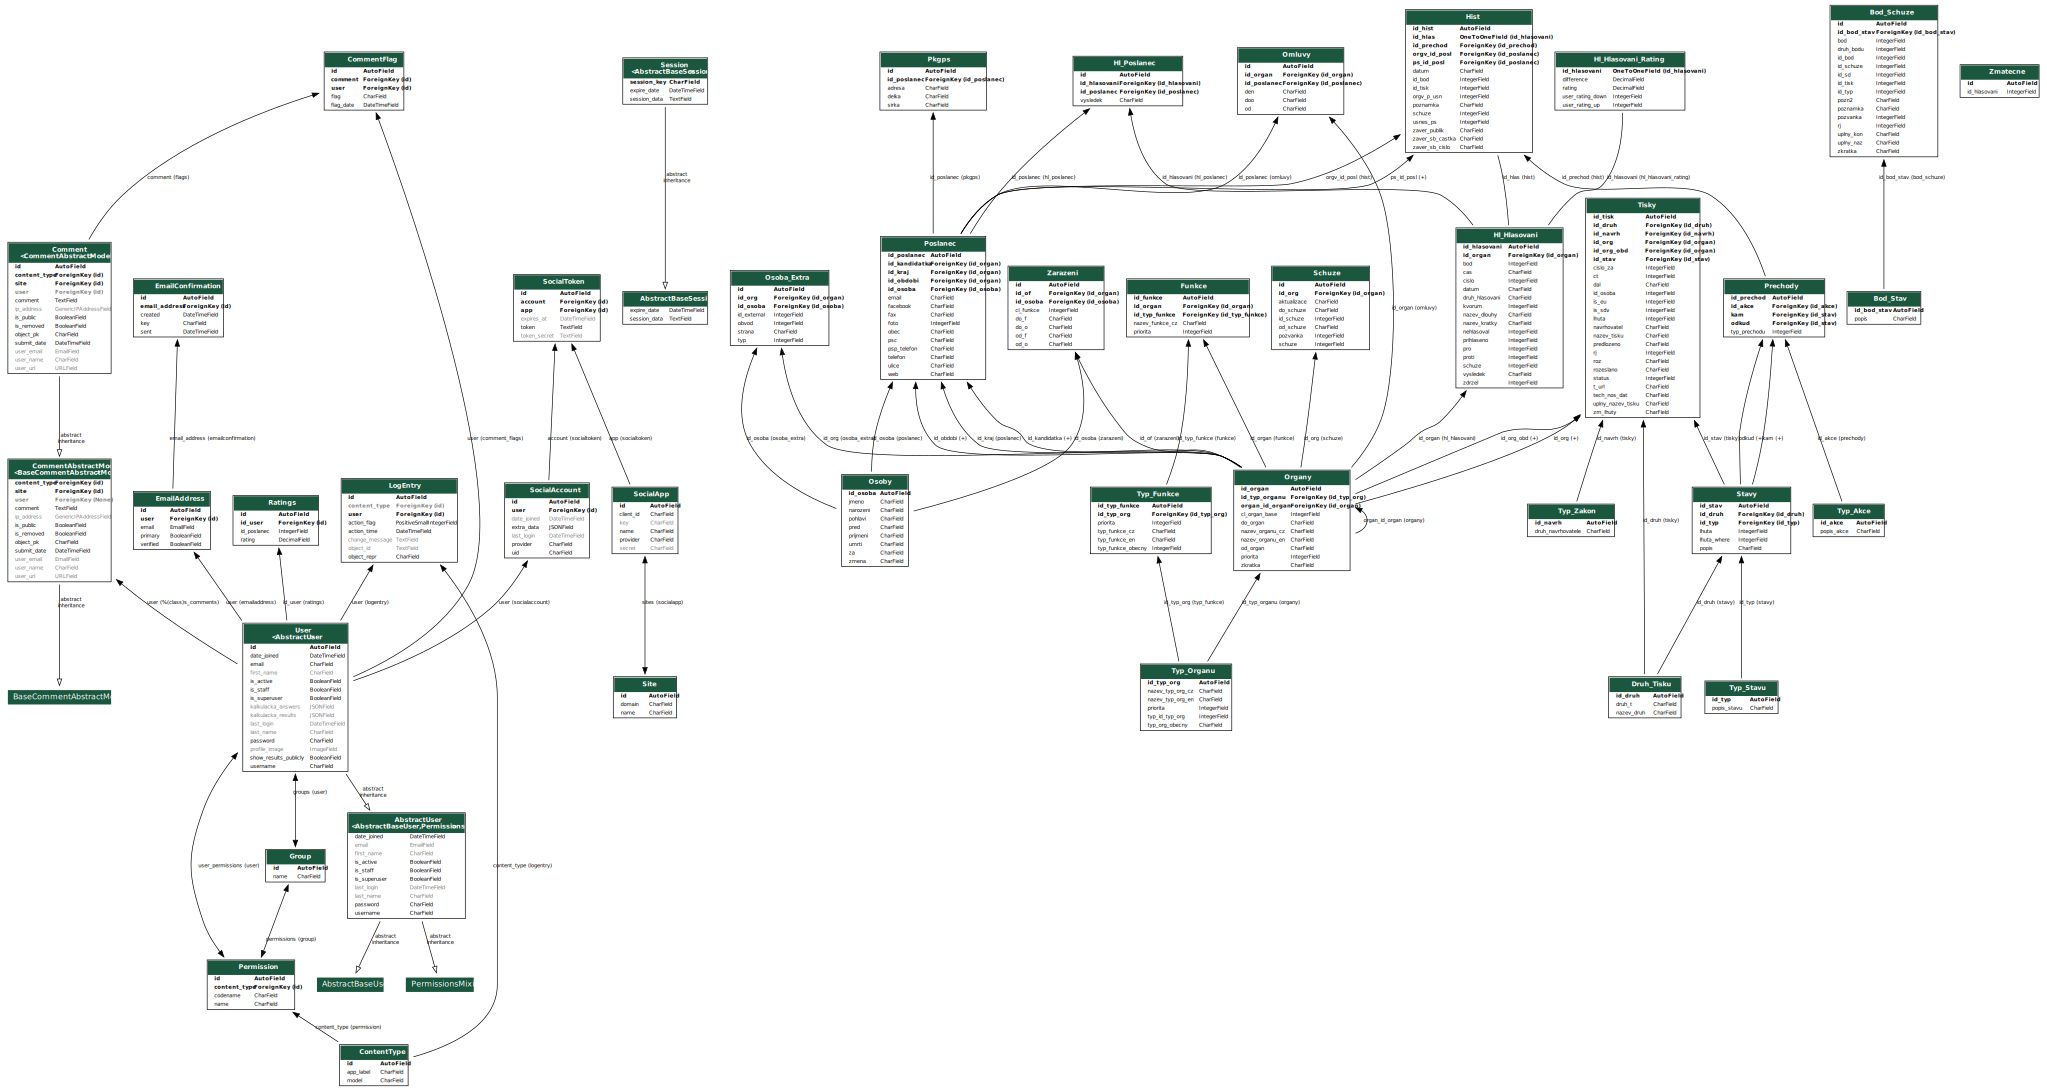
\includegraphics[width=1\textwidth]{obrazky-figures/model-diagram.png}
    \caption{Box plot of number of positions sent per iteration using this scheme}
    \label{fig:awesome_image}
\end{sidewaysfigure}